\documentclass[a4paper, 11pt]{article}
\usepackage{amsmath}
\usepackage{graphicx}
\usepackage{geometry}
\usepackage{listings}
\usepackage{color}
\usepackage{cite}
\usepackage[fontset=ubuntu]{ctex}

\definecolor{dkgreen}{rgb}{0,0.6,0}
\definecolor{gray}{rgb}{0.5,0.5,0.5}
\definecolor{mauve}{rgb}{0.58,0,0.82}
\lstset{frame=shadowbox,
    language=Python,
    aboveskip=3mm,
    belowskip=3mm,
    showstringspaces=false,
    columns=flexible,
    basicstyle={\small\ttfamily},
    numbers=left,
    numberstyle=\tiny\color{gray},
    keywordstyle=\color{blue},
    commentstyle=\color{dkgreen},
    stringstyle=\color{mauve},
    breaklines=true,
    breakatwhitespace=true,
    tabsize=3
}
\usepackage[colorlinks,linkcolor=red]{hyperref}
\geometry{scale=0.8}

\title{	
\normalfont \normalsize
\textsc{School of Data and Computer Science, Sun Yat-sen University} \\ [25pt] %textsc small capital letters
\rule{\textwidth}{0.5pt} \\[0.4cm] % Thin top horizontal rule
\huge Othello Game ($\alpha-\beta$ pruning) \\ % The assignment title
\rule{\textwidth}{2pt} \\[0.5cm] % Thick bottom horizontal rule
\author{17341203 Yixin Zhang}
\date{\normalsize\today}
}

\begin{document}
\maketitle
\tableofcontents
\newpage

\section{Othello}
Othello (or Reversi) is a strategy board game for two players, played on an $8 \times 8$ uncheckered board. There are sixty-four identical game pieces called disks (often spelled "discs"), which are light on one side and dark on the other. Please see figure \ref{fig:othello}.

Players take turns placing disks on the board with their assigned color facing up. During a play, any disks of the opponent's color that are in a straight line and bounded by the disk just placed and another disk of the current player's color are turned over to the current player's color.

The object of the game is to have the majority of disks turned to display your color when the last playable empty square is filled.
\begin{figure}
  \centering
  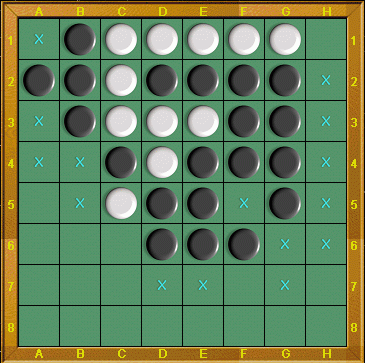
\includegraphics[width=6cm]{Pic/othello}
  \qquad
  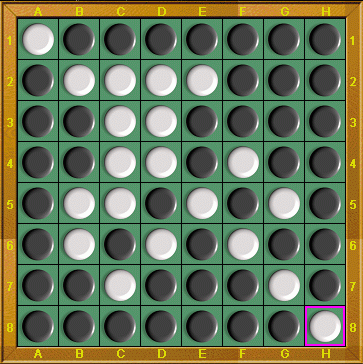
\includegraphics[width=6cm]{Pic/othello2}
  \caption{Othello Game}
  \label{fig:othello}
\end{figure}

You can refer to \url{http://www.tothello.com/html/guideline_of_reversed_othello.html} for more information of guideline, meanwhile, you can download the software to have a try from \url{http://www.tothello.com/html/download.html}. The game installer \texttt{tothello\_trial\_setup.exe} can also be found in the current folder.



\section{Tasks}
\begin{enumerate}

\item In order to reduce the complexity of the game, we think the board is $6\times 6$.

\item There are several evaluation functions that involve many aspects, you can turn to \url{http://blog.sina.com.cn/s/blog_53ebdba00100cpy2.html} for help. In order to reduce the difficulty of the task, I have gaven you some hints of evaluation function in the file \texttt{Heuristic Function for Reversi (Othello).cpp}.

\item Please choose an appropriate evaluation function and use min-max and $\alpha-\beta$ prunning to implement the Othello game. The framework file you can refer to is \texttt{Othello.cpp}. Of course, I wish your program can beat the computer.

\item Write the related codes and take a screenshot of the running results in the file named \textsf{E03\_YourNumber.pdf}, and send it to \textsf{ai\_201901@foxmail.com}.
\end{enumerate}

\section{Codes}

I have read all the codes, and added many comments to help me understand the framework.

Note that I have rearranged the program into three separated files -- `main.cpp', `Othello.h' and `Othello.cpp', so that the code would look clean and tidy.
\begin{lstlisting}[title=main.cpp]
#include <string>
#include "Othello.h"
using namespace std;

const int MAX = 65534;
const int MAX_DEPTH = 10;  //最大搜索深度

/* 最大最小博弈与α-β剪枝 */
Do *minimax(Othello *board, enum Option player, int step, int min, int max, Do *choice) {
    choice->score = -MAX;
    choice->pos.first = -1;
    choice->pos.second = -1;

    int num = board->rule(board, player);  // 找出player可以落子的数量,对应于图像界面里面的‘+’的个数

    // 无处落子
    if (num == 0) {
        // 但对方可以落子,让对方下
        if (board->rule(board, (enum Option) - player) != 0) {
            Othello tempBoard;
            Do nextChoice;
            Do *pNextChoice = &nextChoice;
            board->copy(&tempBoard, board);
            pNextChoice = minimax(&tempBoard, (enum Option) - player, step - 1, -max, -min, pNextChoice);
            choice->score = -pNextChoice->score;
            choice->pos.first = -1;
            choice->pos.second = -1;
            return choice;
        } else {  // 双方都无处落子,游戏结束
            int value = WHITE * (board->white_num) + BLACK * (board->black_num);
            if (player * value > 0) {
                choice->score = MAX - 1;
            } else if (player * value < 0) {
                choice->score = -MAX + 1;
            } else {
                choice->score = 0;
            }
            return choice;
        }
    }

    // 以下都为有处落子的情况

    if (step <= 0)  // 已搜索到最大深度,直接返回得分
    {
        choice->score = board->judge(board, player);  // 评价函数
        return choice;
    }

    // 新建一个Do*类型的数组,其中num即为玩家可落子的数量,用于保存所有可落子的选择
    Do *allChoices = (Do *)malloc(sizeof(Do) * num);

    /****
		下面三个两重for循环其实就是分区域寻找可落子的位置
		,本函数开头的 `num = board->rule(board, player)` 只返
		回了可落子的数量,并没有返回可落子的位置,因此需要重
		新遍历整个棋盘去寻找可落子的位置。
		下面三个for循环分别按照最外一圈、最中间的四个位置、靠
		里的一圈这三个顺序来寻找可落子的位置,如下图所示(数字
		表示寻找的顺序)
		1 1 1 1 1 1
		1 3 3 3 3 1
		1 3 2 2 3 1
		1 3 2 2 3 1
		1 3 3 3 3 1
		1 1 1 1 1 1
	*/
    int k = 0;
    // 最外圈
    for (int i = 0; i < 6; i++) {
        for (int j = 0; j < 6; j++) {
            if (i == 0 || i == 5 || j == 0 || j == 5) {
                /* 可落子的位置需要满足两个条件:1、该位置
                上没有棋子, 2、如果把棋子放在这个位置上可
                以吃掉对方的
				   棋子(可以夹住对方的棋子)。stable记录的是
				   可以吃掉对方棋子的数量,所以stable>0符合条件2
				*/
                if (board->cell[i][j].color == SPACE && board->cell[i][j].stable) {
                    allChoices[k].score = -MAX;
                    allChoices[k].pos.first = i;
                    allChoices[k].pos.second = j;
                    k++;
                }
            }
        }
    }

    // 中间四个位置
    for (int i = 0; i < 6; i++) {
        for (int j = 0; j < 6; j++) {
            if ((i == 2 || i == 3 || j == 2 || j == 3) && (i >= 2 && i <= 3 && j >= 2 && j <= 3)) {
                if (board->cell[i][j].color == SPACE && board->cell[i][j].stable) {
                    allChoices[k].score = -MAX;
                    allChoices[k].pos.first = i;
                    allChoices[k].pos.second = j;
                    k++;
                }
            }
        }
    }

    // 中间圈
    for (int i = 0; i < 6; i++) {
        for (int j = 0; j < 6; j++) {
            if ((i == 1 || i == 4 || j == 1 || j == 4) && (i >= 1 && i <= 4 && j >= 1 && j <= 4)) {
                if (board->cell[i][j].color == SPACE && board->cell[i][j].stable) {
                    allChoices[k].score = -MAX;
                    allChoices[k].pos.first = i;
                    allChoices[k].pos.second = j;
                    k++;
                }
            }
        }
    }

    // 尝试在之前得到的num个可落子位置进行落子
    for (int k = 0; k < num; k++) {
        Do nextChoice;
        Do *pNextChoice = &nextChoice;
        Do thisChoice = allChoices[k];

        Othello tempBoard;
        board->copy(&tempBoard, board);                                                                // 为了不影响当前棋盘,需要复制一份作为虚拟棋盘
        board->action(&tempBoard, &thisChoice, player);                                                // 在虚拟棋盘上落子
        pNextChoice = minimax(&tempBoard, (enum Option) - player, step - 1, -max, -min, pNextChoice);  // 递归调用α-β剪枝,得到对手的落子评分
        thisChoice.score = -pNextChoice->score;                                                        // 上面得到的是对手得分,因此要取相反数

        if (thisChoice.score > min && thisChoice.score < max) /* 可以预计的更优值 */
        {
            min = thisChoice.score;
            choice->score = thisChoice.score;
            choice->pos.first = thisChoice.pos.first;
            choice->pos.second = thisChoice.pos.second;
        } else if (thisChoice.score >= max) /* 好的超乎预计 */
        {
            choice->score = thisChoice.score;
            choice->pos.first = thisChoice.pos.first;
            choice->pos.second = thisChoice.pos.second;
            break;  // 剪枝
        }
        /* 不如已知最优值 */

        /****
            本代码框架与我们在课上学的略有不同。在这里,无论是黑棋
            还是白棋,其得分都是相对自己来说的,不是“MAX节点最大化
            分数、MIN节点最小化分数”的形式,而是双方的目标都是最大
            化自己的分数。其实只需要适当取分数的相反数,即可将这种
            形式转换为我们课上学习的形式。由于上面递归调用中将-max
            和-min分别传参给了min和max,因此可以将MAX节点和MIN节
            点的剪枝代码合二为一,如下。
        */
        // if (thisChoice.score > min) {
        //     min = thisChoice.score;  // 更新alpha的值
        //     choice->score = thisChoice.score;
        //     choice->pos.first = thisChoice.pos.first;
        //     choice->pos.second = thisChoice.pos.second;
        //     if (max <= min) {
        //         break;  // 剪枝
        //     }
        // }
    }

    free(allChoices);
    return choice;
}

int main() {
    Othello board;
    Othello *pBoard = &board;
    enum Option player, present;
    Do choice;
    Do *pChoice = &choice;
    int num, result = 0;
    // char restart = ' ';

    player = SPACE;
    present = BLACK;
    num = 4;
    // restart = ' ';

    cout << ">>> 人机对战开始:" << endl;

    while (player != WHITE && player != BLACK) {
        cout << ">>> 请选择执黑棋(○),或执白棋(●):输入1为黑棋,-1为白棋" << endl;
        scanf("%d", &player);
        cout << ">>> 黑棋行动:  \n";

        if (player != WHITE && player != BLACK) {
            cout << "[-] 输入不符合规范,请重新输入\n";
            player = SPACE;  // 重置
        }
    }

    board.create(pBoard);

    /* BEGIN WHILE */
    while (num < 6 * 6) {  // 棋盘上未下满36个棋子
        string player_str = "";
        if (present == BLACK) {
            player_str = "黑棋(○)";
        } else if (present == WHITE) {
            player_str = "白棋(●)";
        }

        if (board.rule(pBoard, present) == 0)  //未下满并且无子可下
        {
            if (board.rule(pBoard, (enum Option) - present) == 0) {
                break;  // 双方都无子可下
            }
            cout << player_str << "GAME OVER! \n";
        } else {
            int i, j;
            board.show(pBoard);  // 【首先】打印棋盘

            if (present == player) {
                while (1) {
                    cout << player_str << "\n >>> 请输入棋子坐标,先行后列:";
                    cin >> i >> j;
                    i--;
                    j--;  // 转换为数组下标
                    pChoice->pos.first = i;
                    pChoice->pos.second = j;

                    if (i < 0 || i > 5 || j < 0 || j > 5 || pBoard->cell[i][j].color != SPACE || pBoard->cell[i][j].stable == 0) {
                        cout << "[-] 此处落子不符合规则,请重新选择!" << endl;
                        board.show(pBoard);
                    } else {
                        break;
                    }
                }
                CLEARSCREEN;
                cout << ">>> 玩家本手棋得分为:" << pChoice->score << endl;
                PAUSE
                cout << ">>> 按任意键继续..." << pChoice->score << endl;
            } else  //AI下棋
            {
                cout << player_str << "..........................";

                pChoice = minimax(pBoard, present, MAX_DEPTH, -MAX, MAX, pChoice);
                i = pChoice->pos.first;
                j = pChoice->pos.second;

                CLEARSCREEN;

                cout << ">>> AI本手棋得分为     " << pChoice->score << endl;
            }

            board.action(pBoard, pChoice, present);
            num++;
            cout << player_str << ">>> AI于" << i + 1 << "," << j + 1 << "落子,该你了!";
        }

        present = (enum Option) - present;  //交换执棋者
    }
    /* END WHILE */

    /* 游戏结束,打印结果 */
    board.show(pBoard);
    if (pBoard->white_num > pBoard->black_num) {
        cout << "\n—————— 白棋(●)胜 ——————" << endl;
    } else if (pBoard->white_num < pBoard->black_num) {
        cout << "\n—————— 黑棋(○)胜 ——————" << endl;
    } else {
        cout << "\n———————— 平局 ————————" << endl;
    }

    return 0;
}
\end{lstlisting}

\begin{lstlisting}[title=Othello.h]
#ifndef _OTHELLO_H_
#define _OTHELLO_H_
#include <iostream>
using namespace std;

/* 跨平台 */
#define CLEARSCREEN system("clear");
#define PAUSE                               \
    printf("Press any key to continue..."); \
    fgetc(stdin);                           \
    fgetc(stdin);

//基本元素:棋子,颜色,数字变量

enum Option {
    WHITE = -1,
    SPACE,
    BLACK  // 是否能落子  // 黑子
};

struct Do {
    pair<int, int> pos;
    int score;
};

struct WinNum {
    enum Option color;
    int stable;  // 若在此处落子,可以吃掉对方棋子的数量
};

// 主要功能:棋盘及关于棋子的所有操作,功能
class Othello {
   public:
    WinNum cell[6][6];  // 定义棋盘中有6*6个格子
    int white_num;      // 白棋数目
    int black_num;      // 黑棋数目

    void create(Othello *board);                                  // 初始化棋盘
    void copy(Othello *boardDest, const Othello *boardSource);    // 复制棋盘
    void show(Othello *board);                                    // 打印棋盘
    int rule(Othello *board, enum Option player);                 // 计算可以落子的位置数量
    bool action(Othello *board, Do *choice, enum Option player);  // 落子并修改棋盘
    void stable(Othello *board);                                  // 计算赢棋个数
    int judge(Othello *board, enum Option player);                // 计算评价函数
};

#endif
\end{lstlisting}

\begin{lstlisting}[title=Othello.cpp]
#include "Othello.h"
#include <iostream>
using namespace std;

/* 初始化棋盘 */
void Othello::create(Othello *board) {
    int i, j;
    board->white_num = 2;
    board->black_num = 2;
    for (i = 0; i < 6; i++) {
        for (j = 0; j < 6; j++) {
            board->cell[i][j].color = SPACE;
            board->cell[i][j].stable = 0;
        }
    }
    board->cell[2][2].color = board->cell[3][3].color = WHITE;
    board->cell[2][3].color = board->cell[3][2].color = BLACK;
}

/* 复制棋盘 */
void Othello::copy(Othello *Fake, const Othello *Source) {
    int i, j;
    Fake->white_num = Source->white_num;
    Fake->black_num = Source->black_num;
    for (i = 0; i < 6; i++) {
        for (j = 0; j < 6; j++) {
            Fake->cell[i][j].color = Source->cell[i][j].color;
            Fake->cell[i][j].stable = Source->cell[i][j].stable;
        }
    }
}

/* 打印棋盘 */
void Othello::show(Othello *board) {
    cout << "\n  ";
    for (int i = 0; i < 6; i++) {
        cout << "   " << i + 1;
    }
    cout << endl
         << "   ┌───┬───┬───┬───┬───┬───┐" << endl;
    for (int i = 0; i < 6; i++) {  // 每一行
        cout << i + 1 << "--│";
        for (int j = 0; j < 6; j++) {  // 每一列
            switch (board->cell[i][j].color) {
                case BLACK:
                    cout << " ○ │";
                    break;
                case WHITE:
                    cout << " ● │";
                    break;
                case SPACE:
                    if (board->cell[i][j].stable) {
                        cout << " + │";  // 允许落子
                    } else {
                        cout << "   │";  // 不允许落子
                    }
                    break;
                default:  // 棋子颜色错误
                    cout << " ■ │";
            }
        }
        if (i != 5) cout << endl
                         << "   ├───┼───┼───┼───┼───┼───┤" << endl;
    }
    cout << "\n   └───┴───┴───┴───┴───┴───┘\n";

    cout << "    白棋(●)个数为:" << board->white_num << '\t' << "黑棋(○)个数为:" << board->black_num << endl
         << endl;
}

/* 计算可以落子的位置数量 */
int Othello::rule(Othello *board, enum Option player) {
    unsigned num = 0;
    for (int i = 0; i < 6; i++) {
        for (int j = 0; j < 6; j++) {
            if (board->cell[i][j].color == SPACE) {  // 遍历整个棋盘上的空cell
                board->cell[i][j].stable = 0;
                for (int x = -1; x <= 1; x++) {
                    for (int y = -1; y <= 1; y++) {
                        // 8个方向
                        if (x != 0 || y != 0) {
                            unsigned num2 = 0;
                            for (int i2 = i + x, j2 = j + y; i2 >= 0 && i2 < 6 && j2 >= 0 && j2 < 6; i2 += x, j2 += y) {
                                // 当前检查的cell是对方的棋子
                                if (board->cell[i2][j2].color == (enum Option) - player) {
                                    num2++;
                                } else if (board->cell[i2][j2].color == player) {
                                    board->cell[i][j].stable += player * num2;
                                    break;
                                } else if (board->cell[i2][j2].color == SPACE) {
                                    break;
                                }
                            }
                        }
                    }
                }

                if (board->cell[i][j].stable) {
                    num++;
                }
            }
        } /* END FOR J */
    }     /* END FOR I */
    return num;
}

/* 落子并修改棋盘 */
bool Othello::action(Othello *board, Do *choice, enum Option player) {
    int i = choice->pos.first, j = choice->pos.second;  // 准备落子的位置

    // 若准备落子的位置上已经有棋子,或者在这个位置落子
    // 不能吃掉对方任何棋子的话,说明这个action无效
    if (board->cell[i][j].color != SPACE || board->cell[i][j].stable == 0 || player == SPACE) {
        return false;  // 落子无效
    }

    board->cell[i][j].color = player;
    board->cell[i][j].stable = 0;

    // 更新棋子数量
    if (player == WHITE) {
        board->white_num++;
    } else if (player == BLACK) {
        board->black_num++;
    }

    for (int x = -1; x <= 1; x++) {
        for (int y = -1; y <= 1; y++) {
            // 需要在8个方向上检测落子是否符合规则(能否吃子)
            if (x != 0 || y != 0) {
                unsigned num = 0;
                for (int i2 = i + x, j2 = j + y; i2 >= 0 && i2 <= 5 && j2 >= 0 && j2 <= 5; i2 += x, j2 += y) {
                    if (board->cell[i2][j2].color == (enum Option) - player) {
                        num++;
                    } else if (board->cell[i2][j2].color == player) {
                        board->white_num += (player * WHITE) * num;
                        board->black_num += (player * BLACK) * num;

                        for (i2 -= x, j2 -= y; num > 0; num--, i2 -= x, j2 -= y) {
                            board->cell[i2][j2].color = player;
                            board->cell[i2][j2].stable = 0;
                        }
                        break;
                    } else if (board->cell[i2][j2].color == SPACE) {
                        break;
                    }
                }
            }
        }
    }
    return true;  // 落子有效
}

/* 计算赢棋个数 */
void Othello::stable(Othello *board) {
    for (int i = 0; i < 6; i++) {
        for (int j = 0; j < 6; j++) {
            if (board->cell[i][j].color != SPACE) {
                board->cell[i][j].stable = 1;

                for (int x = -1; x <= 1; x++) {
                    for (int y = -1; y <= 1; y++) {
                        // 4个方向
                        if (x == 0 && y == 0) {
                            x = 2;
                            y = 2;
                        } else {
                            int flag = 2;
                            for (int i2 = i + x, j2 = j + y; i2 >= 0 && i2 <= 5 && j2 >= 0 && j2 <= 5; i2 += x, j2 += y) {
                                if (board->cell[i2][j2].color != board->cell[i][j].color) {
                                    flag--;
                                    break;
                                }
                            }

                            for (int i2 = i - x, j2 = j - y; i2 >= 0 && i2 <= 5 && j2 >= 0 && j2 <= 5; i2 -= x, j2 -= y) {
                                if (board->cell[i2][j2].color != board->cell[i][j].color) {
                                    flag--;
                                    break;
                                }
                            }

                            /* 在某一条线上稳定 */
                            if (flag != 0) {
                                board->cell[i][j].stable++;
                            }
                        }
                    }
                }
            }
        }
    }
}

/* 计算评价函数 */
int Othello::judge(Othello *board, enum Option player) {
    stable(board);
    int value = 0;

    // 对稳定子给予奖励
    // for (int i = 0; i < 6; i++) {
    //     for (int j = 0; j < 6; j++) {
    //         if(board->cell[i][j].color == player) {
    //             value += 10 * board->cell[i][j].stable;  // 是自己就奖励
    //         }
    //         else if(board->cell[i][j].color == (enum Option) - player) {
    //             value -= 10 * board->cell[i][j].stable;  // 是对方就惩罚
    //         }
    //     }
    // }

    double d = 0;
    int my_tiles = 0, opp_tiles = 0, my_front_tiles = 0, opp_front_tiles = 0;

	int X1[] = {-1, -1, 1, 1, 0, -1};
	int Y1[] = {0, 1, 1, 0,  -1, -1};
    int V[6][6] = {
        {20, -5, 8, 8, -5, 20},
        {-5, -7, 1, 1, -7, -5},
        {8, 1, -3, -3, 1, 8},
        {8, 1, -3, -3, 1, 8},
        {-5, -7, 1, 1, -7, -5},
        {20, -5, 8, 8, -5, 20}};

    for (int i = 0; i < 6; i++) {
        for (int j = 0; j < 6; j++) {
            if (board->cell[i][j].color == player) {  // 奖励自己
                d += V[i][j];
                my_tiles++;
            } else if (board->cell[i][j].color == (enum Option) - player) {  // 惩罚对方
                d -= V[i][j];
                opp_tiles++;
            }
            // if (board->cell[i][j].color != SPACE) {
            //     for (int k = 0; k < 6; k++) {
            //         int x = i + X1[k];
            //         int y = j + Y1[k];
            //         if (x >= 0 && x < 6 && y >= 0 && y < 6 && board->cell[i][j].color == SPACE) {
            //             if (board->cell[i][j].color == player)
            //                 my_front_tiles++;
            //             else
            //                 opp_front_tiles++;
            //             break;
            //         }
            //     }
            // }
        }
    } /* END FOR */

    double p = 0;
    if (my_tiles > opp_tiles)
        p = (100.0 * my_tiles) / (my_tiles + opp_tiles);
    else if (my_tiles < opp_tiles)
        p = -(100.0 * opp_tiles) / (my_tiles + opp_tiles);
    else
        p = 0;

    double f = 0;
    // if (my_front_tiles > opp_front_tiles)
    //     f = -(100.0 * my_front_tiles) / (my_front_tiles + opp_front_tiles);
    // else if (my_front_tiles < opp_front_tiles)
    //     f = (100.0 * opp_front_tiles) / (my_front_tiles + opp_front_tiles);
    // else
    //     f = 0;

    // 行动力
    double m = 0;
	my_tiles = rule(board, player);
	opp_tiles = rule(board, (enum Option) - player);
	if(my_tiles > opp_tiles)
		m = (75.0 * my_tiles)/(my_tiles + opp_tiles);
	else if(my_tiles < opp_tiles)
		m = -(75.0 * opp_tiles)/(my_tiles + opp_tiles);
	else m = 0;

    value += (10 * p) + (78.922 * m) + (74.396 * f);

    return value;  // 该分数对player来说越大(越正)越好
}
\end{lstlisting}

\section{Results}

\begin{figure}[ht]
  \centering
  
\includegraphics[width=6cm]{Pic/1}
  \qquad
  
\includegraphics[width=6cm]{Pic/2}
  \caption{Othello Game}
  \label{fig:othello}
\end{figure}

It is hard to beat the computer since it is really smart and strong. And due to the tight deadline of this experiment, I don't have enough time to design a great evaluation function. In the future, I will try improving my algorithm in order to make it perform much better.

%\clearpage
%\bibliography{E:/Papers/LiuLab}
%\bibliographystyle{apalike}
\end{document} 